\documentclass[11pt]{article}
% Shared preamble for the preseason 2026 articles. House style follows papers/queta.tex.
\usepackage[margin=1in]{geometry}
\usepackage{amsmath,amssymb}
\usepackage{booktabs}
\usepackage{graphicx}
\usepackage{xcolor}
\usepackage{multirow}
\usepackage{pgfplots}
\pgfplotsset{compat=1.17}
\usepgfplotslibrary{groupplots}
\usepackage{caption}
\captionsetup{font=small,labelfont=bf}
\usepackage[colorlinks=true,linkcolor=black,citecolor=black,urlcolor=blue!50!black]{hyperref}
\usepackage{microtype}
\usepackage{xurl}
\usepackage{enumitem}
\usepackage{float}

\definecolor{court}{HTML}{0E5A3A}
\definecolor{amberx}{HTML}{B26A1F}
\definecolor{steel}{HTML}{5E6E75}
\definecolor{fade}{HTML}{AEB3B5}

\newcommand{\gravity}{\textsc{gravity}}
\newcommand{\ctg}{\textsc{ctg}}
\newcommand{\plainbox}[1]{\par\medskip\noindent\begin{center}%
\colorbox{court!8}{\parbox{0.93\textwidth}{\small \textbf{\textcolor{court}{In plain terms:}} #1}}%
\end{center}\medskip}

% Inline source marker: \src{n}{url} prints a linked superscript [n].
\newcommand{\src}[2]{\textsuperscript{\href{#2}{[#1]}}}

\usepackage{fancyhdr}
\newcommand{\statusfoot}{%
  \fancyhf{}%
  \fancyfoot[L]{\footnotesize\textcolor{steel}{An article, not a research paper}}%
  \fancyfoot[C]{\thepage}%
  \fancyfoot[R]{\footnotesize\textcolor{steel}{thegravityreport.com}}%
  \renewcommand{\headrulewidth}{0pt}%
  \renewcommand{\footrulewidth}{0pt}%
}
\fancypagestyle{gravity}{\statusfoot}
\fancypagestyle{plain}{\statusfoot}
\pagestyle{gravity}

% Version line required at the top of every preseason article.
\newcommand{\versionline}[1]{\par\noindent\begin{center}%
\colorbox{fade!25}{\parbox{0.93\textwidth}{\centering\small
\textbf{v1 --- methodology and figures verified against public sources as of #1.
This article will be revised.}\\[2pt]
Not a research paper: an article, typeset in \LaTeX. Independent analysis, not peer reviewed.}}%
\end{center}\smallskip}

\newcommand{\betbox}[1]{\par\medskip\noindent\begin{center}%
\fcolorbox{court}{court!6}{\parbox{0.93\textwidth}{\small #1}}%
\end{center}\medskip}

\setlist{nosep,leftmargin=1.4em}
\setlength{\emergencystretch}{3em}

% Forecast display: plain-text claim, a bar filled to the probability, a tick at 50% (coin flip).
% Usage: \forecastitem{50}{Claim text.}{Grading note.}
\newcommand{\forecastscale}{%
  \par\noindent\begin{tikzpicture}
  \node[font=\scriptsize, text=steel, anchor=west] at (0,0) {0\%};
  \node[font=\scriptsize, text=steel] at (4.5,0) {coin flip};
  \node[font=\scriptsize, text=steel, anchor=east] at (9,0) {100\%};
  \end{tikzpicture}\par\vspace{-2pt}}
\newcommand{\forecastitem}[3]{%
  \par\medskip\noindent{\small\textbf{#2}}\par\vspace{3pt}\noindent
  \begin{tikzpicture}[baseline=(b.base)]
  \fill[fade!30] (0,0) rectangle (9,0.34);
  \fill[court!80] (0,0) rectangle ({9*#1/100},0.34);
  \draw[steel, line width=0.6pt] (4.5,-0.07) -- (4.5,0.41);
  \node[anchor=west, font=\large\bfseries, text=court] (b) at (9.25,0.17) {#1\%};
  \end{tikzpicture}%
  \ifx\relax#3\relax\else\par\vspace{1pt}\noindent{\footnotesize\textcolor{steel}{#3}}\fi\par}

\newcommand{\puretop}{(1980,5) (1981,9) (1982,7) (1983,8) (1984,6) (1985,5) (1986,3) (1987,3) (1988,2) (1989,4) (1990,2) (1991,3) (1992,4) (1993,4) (1994,4) (1995,3) (1996,1) (1997,2) (1998,4) (1999,6) (2000,5) (2001,3) (2002,3) (2003,2) (2004,2) (2005,4) (2006,1) (2007,2) (2008,2) (2009,4) (2010,3) (2011,2) (2012,2) (2013,1) (2014,2) (2015,4) (2016,0) (2017,0) (2018,0) (2019,0) (2020,0) (2021,0) (2022,0) (2023,0) (2024,0) (2025,0) (2026,1)}
\newcommand{\nstop}{(1980,10) (1981,10) (1982,10) (1983,10) (1984,10) (1985,10) (1986,8) (1987,8) (1988,8) (1989,7) (1990,6) (1991,5) (1992,6) (1993,4) (1994,5) (1995,4) (1996,3) (1997,3) (1998,5) (1999,6) (2000,7) (2001,5) (2002,5) (2003,3) (2004,3) (2005,5) (2006,3) (2007,3) (2008,3) (2009,4) (2010,3) (2011,2) (2012,3) (2013,2) (2014,2) (2015,4) (2016,0) (2017,0) (2018,0) (2019,0) (2020,0) (2021,0) (2022,0) (2023,0) (2024,3) (2025,1) (2026,1)}


\title{\textbf{The Last of His Kind}\\[4pt]
\large For ten seasons no player who refused to shoot threes was in the top ten,\\
until Jalen Duren.\\[2pt]
\normalsize A Gravity Report Deep Dive}
\author{}
\date{October 13, 2026}

\begin{document}
\maketitle
\vspace{-2.5em}
\versionline{October 13, 2026}

\begin{abstract}
\noindent
Every other player in our top ten last season took at least 22\% of his shots from three.
Jalen Duren took none of them, and our per-minute rating still put him as the 7th best player
in the league. That hasn't happened in over a decade. From 2015 to 2025, there wasn't a single
player who never shot threes that finished in the top ten. Back in the 2004--05 season there
were four of them, including the best player in the league. Today we look at how that kind of
player has disappeared, how Duren is a top player without having a skill that is more
important than ever in the modern game, and why we rank him 14th. Duren and the Pistons were
in a four-month-long contract standoff, but now that it's finally over and he's getting paid
\$200 million over the next five years, we give it an \textbf{80\%} chance that he finishes
top 15 next July.
\end{abstract}

\section*{The top ten, and the odd one out}

\begin{table}[h]
\centering\small
\caption{Our ten best players per minute in 2025--26 (\gravity{} Historical, 1,500+ minutes), with
their impact rating and the share of shots they take from three.}
\begin{tabular}{rlcc}
\toprule
& Player & Impact & Three-point attempt rate \\
\midrule
1 & Nikola Jokić & $+3.45$ & .261 \\
2 & Shai Gilgeous-Alexander & $+3.30$ & .226 \\
3 & Victor Wembanyama & $+2.82$ & .324 \\
4 & Luka Dončić & $+2.57$ & .476 \\
5 & Kawhi Leonard & $+2.17$ & .354 \\
6 & Cade Cunningham & $+1.71$ & .308 \\
7 & \textbf{Jalen Duren} & $\mathbf{+1.61}$ & \textbf{.000} \\
8 & Donovan Mitchell & $+1.48$ & .439 \\
9 & Tyrese Maxey & $+1.42$ & .399 \\
10 & LaMelo Ball & $+1.29$ & .595 \\
\bottomrule
\end{tabular}
\label{tab:top10}
\end{table}

The list above is the modern NBA summarized. Even the two centers ranked above Duren shoot.
Jokić takes a quarter of his shots from three, and Wembanyama takes a third. Duren's
three-point attempt rate rounds to zero (he didn't take a single
one).\src{1}{https://www.basketball-reference.com/leagues/NBA_2026_advanced.html}

One note on the ranking itself. Table~\ref{tab:top10} uses \gravity{} Historical, our
per-minute rating: the same formula behind Deep Dives No.~1 and No.~2, minus the on/off numbers we license from
Cleaning the Glass, which only go back to 2003--04 and can't be published. Leaving that input
out lets us run the exact same rating on every season since 1977--78 and line Duren's season
up against Garnett's or Shaq's.\src{2}{https://www.basketball-reference.com/leagues/} It's
also why this table can have Duren 7th while we rank him 14th overall: The 644 starts from
this rating, adds the on/off input, blends in the season before, and charges or credits the
playoffs.

\section*{Ten years without one}

When the three-point line was first introduced in 1979, nearly every regular player ignored
it. In 2014--15, about 29\% of players with 1,500 minutes still took less than one in ten of
their shots from three. As of last season that cohort has dropped to just 6\% of the league.

The best players changed faster than the rest. Figure~\ref{fig:extinct} shows the pure
non-shooters (taking 2\% or less of their shots from three) among every season's ten best
players.

\begin{figure}[h]
\centering
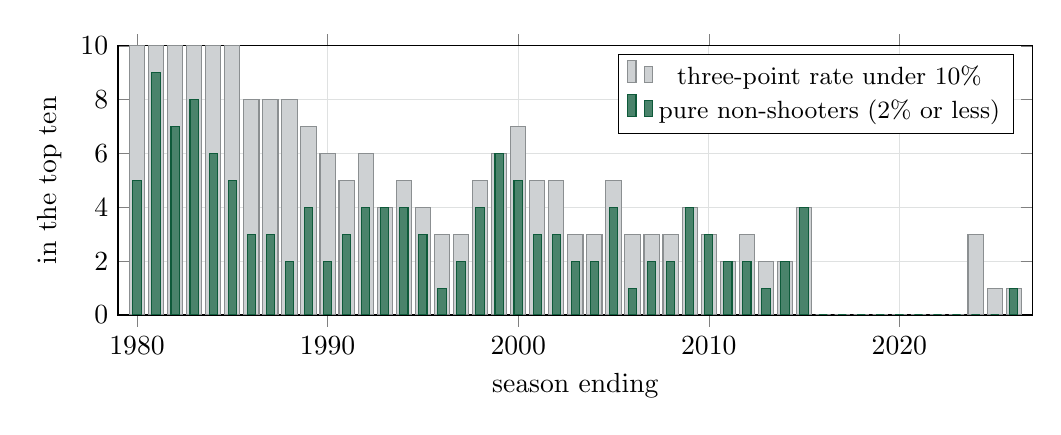
\begin{tikzpicture}
\begin{axis}[
  width=13.2cm, height=5.0cm, ybar, bar width=5.5pt,
  xmin=1979, xmax=2027, ymin=0, ymax=10,
  xlabel={season ending}, ylabel={in the top ten},
  xtick={1980,1990,2000,2010,2020}, x tick label style={/pgf/number format/1000 sep=},
  ytick={0,2,4,6,8,10}, grid=major, grid style={fade!40},
  legend style={font=\small, at={(0.98,0.97)}, anchor=north east},
]
\addplot[fill=fade!60, draw=fade!80!black, bar shift=0pt] coordinates {\nstop};
\addplot[fill=court!75, draw=court, bar shift=0pt, bar width=3pt] coordinates {\puretop};
\legend{three-point rate under 10\%, pure non-shooters (2\% or less)}
\end{axis}
\end{tikzpicture}
\caption{Non-shooters among each season's ten best players per minute, 1979--80 to
2025--26. The single green bar all the way to the right is Duren.}
\label{fig:extinct}
\end{figure}

In 2004--05, four of the top ten were pure non-shooters: Kevin Garnett, who ranked first that
year, Tim Duncan, Shaquille O'Neal, and a 22-year-old Amar'e Stoudemire. In 2014--15 there
were still four of them: Anthony Davis, Duncan, Marc Gasol, and DeMarcus Cousins. The
following season that count dropped to zero and stayed there for ten straight seasons. The
larger group (players under a 10\% rate) did see a return in 2023--24 and the next season
after that through Giannis Antetokounmpo, Domantas Sabonis, and Anthony Davis. However, all
three of them at least shoot a little. Duren doesn't shoot at all.

Duren's season also belongs on an interesting historical list. Since 1979--80, only eight
seasons by players aged 22 or younger have been rated higher without shooting threes: Davis
(again), Shaq twice, Michael Jordan, Magic Johnson, Tracy McGrady, Zion Williamson, and Isiah
Thomas.

\section*{How does he do it?}

\begin{table}[h]
\centering\small
\caption{Duren's season by component. Each value shown is a z-score against the
league-average minute: zero is average and +1 is one standard deviation better.}
\setlength{\tabcolsep}{5pt}
\begin{tabular}{ccccccccc}
\toprule
Box & WinSh & Volume & Effic. & Creation & Load & Stocks & Rebound & Rim \\
\midrule
$+1.63$ & $\mathbf{+2.79}$ & $+1.43$ & $\mathbf{+2.60}$ & $-0.59$ & $+0.18$ & $+0.38$ & $\mathbf{+2.57}$ & $\mathbf{+2.26}$ \\
\bottomrule
\end{tabular}
\label{tab:z}
\end{table}

A good jump shot is one way to be efficient, but Duren found others. His true shooting was
.688 on a 23.6\% usage rate, which comes out to 2.6 standard deviations above the
league-average minute once you look at how much of the offensive burden landed on him. He
grabbed 20.9\% of available rebounds and drew a free-throw attempt for every two shots he
took.\src{3}{https://www.basketball-reference.com/players/d/durenja01.html} All four of
those parts of his game, efficiency, win shares, rebounding, and rim pressure, sit more than
two standard deviations above average. The weak spot shows up in creation, where he comes in
at below average. He doesn't run an offense, but he completes a very good one paired with Cade
Cunningham, who ranks 6th on the same list.

Among the 164 players with over 1,500 minutes, Duren ranked the best in efficiency under
load, third in win shares per 48 minutes, fourth in rim pressure, and fifth in rebounding.
Another way to say this is that Duren's value is concentrated in the very few square feet the
three-point revolution left for centers to work in, and nobody was more efficient than him
there.

Cleaning the Glass, which filters out garbage time, fills in some of the details. 72\% of
Duren's shots happened at the rim, which is more than 82\% of bigs, and we already know none
of them came from three. He scored 137.5 points per 100 shot attempts, placing him in the 93rd
percentile, and he drew a shooting foul on 22.5\% of his shots, which is in the 95th
percentile. He also rebounded 14.1\% of his teammates' missed shots. However, there was one
job that the old center always had that we couldn't find in the case of Duren. His block rate
of 1.5\% puts him in the 49th percentile for
bigs.\src{8}{https://cleaningtheglass.com/stats/player/5102} He's an offense-first center.

\section*{Why we rank him 14th}

We rank Duren 14th overall, seven places below his spot in Table~\ref{tab:top10}, and the
reason is almost entirely the playoffs. Duren's playoff BPM of $-1.7$ in 422 minutes against
Cleveland and Orlando was 6.7 points lower than his regular season, and the model's playoff
weighting hit the lowest it can go. That alone costs him 4.3 points of gravity score. Of all
229 players in The 644 who played in the postseason, he was the only one to hit that
mark.\src{4}{https://thegravityreport.com/notes/spec/}\textsuperscript{,}\src{5}{https://thegravityreport.com/the644/the644-2026-07.csv}

His playoff numbers show exactly what fell apart. 70\% of his shots still left his hands at
the rim, but he only drew fouls on 11.8\% of them, half of his regular-season rate, and his
short mid-range shot percentage dropped to 22\% compared to his regular 50\%, a major
decrease. To top it off, his points per 100 shot attempts came down from 137.5 to 110.0, the
26th percentile for playoff bigs.\src{8}{https://cleaningtheglass.com/stats/player/5102}
Excluding the playoffs, he would climb up to 8th in our rankings.

The rest of the gap is pretty small. The full model grades his regular season slightly lower,
at +1.51 instead of +1.61, because it includes the on/off input and has slightly different
skill weights.

We hear a lot of talk about how fans don't want to pay so much for a player who can't perform
on the biggest stage. The poor end to last season has left a bad taste in the mouths of
Pistons fans going into this offseason, and it has blinded them from seeing what a great
player he really was all year long. It may also raise some concerns for the next playoff run,
but that's a conversation for later. Duren will definitely help Detroit run a successful
campaign in a competitive East.

\section*{The contract}

When we first started writing this article, Duren was still unsigned, and we were a little
unsure of his future. He had turned down a five-year, \$200 million deal and skipped media
day, and his qualifying offer of \$9.6 million was set to expire on October
1st.\src{6}{https://www.espn.com/nba/story/_/id/50051681/sources-pistons-duren-not-media-day-amid-contract-standoff}
He decided to take the long-term deal that same day, before the 11:59 p.m. deadline. ESPN
reported that he had objected to weight clauses in Detroit's earlier
offers.\src{7}{https://www.espn.com/nba/story/_/id/50081576/jalen-duren-accepts-5-year-200m-deal-pistons-agent-says}
Even though he did miss media day and the first few practices of camp, Detroit fans can sleep
at night knowing that their star center won't be sitting out games over a contract.

\section*{The forecast}

Throughout history, young centers tend to stay good. Of the 22 seasons since 1977--78 from
centers aged 21 to 23 with a comparable rating to Duren's, 18 of them were followed by a year
that would keep Duren in the top 15. If he has an exact repeat of last season, his gravity score would rise to 71.1,
which would rank him 7th.

Now that his contract issues have been resolved, we give it an 80\% chance that he stays in
the top 15. Injury would be the main risk
that threatens this.

Our external prediction revolves around that traditional-center title. Since 1999--00, the
best BPM among centers with a three-point attempt rate under 10\% has gone to the same player
in back-to-back seasons 11 out of 26 times. Duren led that group last year, and we give him a
60\% chance to repeat, because Alperen Şengün took under 10\% of his shots from three as
recently as 2024--25 and could easily qualify for this again.

\forecastscale
\forecastitem{80}{Jalen Duren ranks top 15 in The 644, July 2027 edition.}{\#1--15 = Win \quad
\#16--20 = Near miss (graded as a miss) \quad \#21 or below = Miss. This is our own ranking;
we keep one bet on it each article so the model gets graded too.}
\forecastitem{60}{Jalen Duren posts the highest 2026--27 BPM among players listed at center with
a three-point attempt rate below 10\% and 1,500+ regular-season minutes.}{Basketball Reference,
final regular-season table.}

\medskip\noindent{\footnotesize\textcolor{steel}{External predictions are graded on Basketball
Reference's final regular-season tables by April 30, 2027. Registered October 17, 2026, before
the October 18 freeze. Scored by Brier score in the Forecast Ledger.}}

\enlargethispage{1\baselineskip}
\section*{Method and sources}
\footnotesize
\gravity{} Historical (\gravity-RS in the code) per the specification's retrospective equation, 1977--78
to 2025--26; three-point attempt rate from Basketball Reference advanced tables. ``Pure
non-shooter'': three-point attempt rate of 2\% or less. Code: \texttt{papers/duren/} (\texttt{extinct.py}, \texttt{analysis.py}) and
\texttt{papers/common/} (\texttt{gravity\_rs.py}, \texttt{pipeline.py}).
\begin{enumerate}[label={[\arabic*]},nosep]
\item Basketball Reference, 2025--26 advanced table. \url{https://www.basketball-reference.com/leagues/NBA_2026_advanced.html}
\item Basketball Reference, league advanced and per-100 tables, 1977--78 to 2025--26. \url{https://www.basketball-reference.com/leagues/}
\item Basketball Reference, Jalen Duren. \url{https://www.basketball-reference.com/players/d/durenja01.html}
\item The Gravity Report, The \gravity{} Specification, v3. \url{https://thegravityreport.com/notes/spec/}
\item The Gravity Report, The 644, July 2026 edition (CSV). \url{https://thegravityreport.com/the644/the644-2026-07.csv}
\item ESPN, Duren not at media day amid contract standoff, September 28, 2026. \url{https://www.espn.com/nba/story/_/id/50051681/sources-pistons-duren-not-media-day-amid-contract-standoff}
\item ESPN, Duren accepts five-year, \$200 million deal, October 1, 2026. \url{https://www.espn.com/nba/story/_/id/50081576/jalen-duren-accepts-5-year-200m-deal-pistons-agent-says}
\item Cleaning the Glass, Jalen Duren (garbage time filtered; percentiles by position), accessed September 29, 2026. \url{https://cleaningtheglass.com/stats/player/5102}
\end{enumerate}

\end{document}
